\section{Overview}
Industrial control system (ICS) is a generic term for the broad class of automation systems associated with controlling and monitoring of manufacturing and industrial facilities. A Programmable Logic Controller (PLC) is an industrial digital computer used to control the manufacturing processes. Traditionally, discussions concerning ICS and PLCs refer to the control systems that regulate critical infrastructure. 


\subsection{Information Technology vs Operational Technology}
Information Technology (IT) refers to the use of systems (especially computers) to store, retrieve and send information. Operational Technology (OT) refers to the hardware and software to operate Industrial Control Systems. OT differs from IT in that OT (1) has a much longer lifespan (10 years) (2) is designed with improved shock resistance (3) runs with little human interaction (4) requires 100\% availability.


\subsection{Understanding PLCs}
A PLC contains a CPU, for logic and processing, memory, and input/output circuits. A running PLC continually scans a program. The scanning cycle is composed of three phases: (1) Checking inputs - the PLC will read information from any connected sensors (2) Execute Program Logic - the PLC will execute the uploaded program logic (3) Writing outputs - the PLC will write to the output devices (actuators) based on the executed logic.


\subsection{IEC-61131-3 Standard Protocol}
The International Electrotechnical Commission (IEC) 61131-3 standard protocol specifies how PLCs are  manufactured and programmed. IEC-61131-3 specifically defines the five programming languages supported by PLCs. The defined languages are (1) Ladder Diagrams (LD), (2) Function Block Diagram (FBD), (3) Structured Text (ST), (4) Instruction List (IL), and (5) Sequential Function Chart (SFC). This lab uses the most popular programming language for PLCs, Ladder Diagrams also known as Ladder Logic.


\subsection{Lab Environment} 
Figure~\ref{fig:labsetup} depicts the lab environment. 

\begin{figure}[!htb]
\begin{center}
\tcbox[colframe=black,colback=white!30]{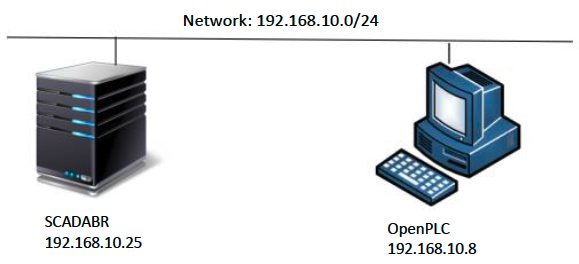
\includegraphics[width=.81\textwidth]{./images/OneLAN_OneHost.png}}
\end{center}
\caption{Lab Environment}
\label{fig:labsetup}
\end{figure}

In this lab, you will use two machines that are connected to the same LAN. The ICS Security machine contains the OpenPLC editor software, for creating and editing ladder diagrams, and the OpenPLC runtime software, which executes the ladder logic created from the OpenPLC editor.The SCADABR machine executes the HMI builder software. The SCADABR machine runs in the background.  The HMI builder software is accessed using the OpenPLC machine, via a standard web browser using the SCADABR IP address and port 8080. For this lab the URL to access the HMI Builder software is http://192.168.10.25:8080/ScadaBR.  


\subsection{Lab Objectives}
There are four objectives for this lab 
\begin{enumerate} [noitemsep]
\item introduce Industrial Control Systems
\item introduce Programmable Logic Controllers
\item introduce Programming with Ladder Diagrams
\item write simple ladder diagram programs
\end{enumerate}